\chapter{Experiment}\label{chap:experiment}
\begin{jointwork}
    The apparatus description took contents from Ref.\,\cite{Walter2025_CASPErLFthermal}.
    Sections~\ref{sec:experiment:sensitivity}--\ref{sec:experiment:scanning} are partially adapted from Ref.\,\cite{Yuzhe2023_FrequencyScanning} and Ref.\,\cite{YGK2026_CavityLumpedSpin}.
\end{jointwork}

The CASPEr-Gradient-Lowfield apparatus converts a nuclear-spin signal into a detectable electrical output through three functional blocks: the magnet system sets the operating bias magnetic field and thereby the Larmor frequency of the sample; the sample and pickup coil generate and capture the magnetic response; and the SQUID and lock-in amplifier chain convert, amplify, and record the signal.
This chapter describes each block, summarizes the key parameters, and then develops the strategy used to scan an ALP-mass range efficiently.

\section{Apparatus}\label{sec:apparatus}
\subsection{Cryostat and magnet}\label{sec:apparatus:magnet}

The apparatus is built around a flow-through L\ch{He} cryostat inside a Faraday room, shielded from external electric fields.
It consists of an outer shell, reservoirs for liquid nitrogen (L\ch{N2}) and L\ch{He}, and vacuum insulation layers in between.
L\ch{N2} cools the cryostat and reduces the evaporation of L\ch{He}, while the superconducting devices and niobium (\ch{Nb}) shield are submerged in the L\ch{He} bath at \SI{4.2}{\kelvin}. 
When fully filled, the cryostat can maintain a superconducting environment for approximately one week.
The \ch{Nb} shield repels external magnetic fields (Meissner effect), isolating internal devices from external magnetic noise.
% A superconducting \ch{Nb} shield built into the cryostat attenuates low-frequency magnetic noise.
Additional shielding is provided by a $\mu$-metal shield outside the cryogenic reservoir and by a Faraday cage enclosing the entire apparatus, which suppresses electromagnetic interference (EMI).


The cryostat houses a superconducting solenoid that can generate a bias magnetic field $B_0$ up to \SI{0.1}{\tesla}.
The DM mass range accessible to the experiment depends on the gyromagnetic ratio of the sample and on $B_0$; for proton spins, the covered Larmor frequency range goes up to \SI{4.3}{\MHz}. 

Eight superconducting shim coils (named Z1, Z2, X, Y, XY, XZ, YZ, and X$^2$-Y$^2$) surrounding the solenoid are used to reduce the field inhomogeneity to less than \SI{2}{\ppm} over a spherical volume with radius \SI{4}{\mm}.
The shim coil channel names indicate the geometry of the magnetic field they generate, enabling systematic correction of field inhomogeneities. 
In the measurements reported here, an inhomogeneity of approximately \SI{10}{\ppm} was achieved after tuning the shim fields using a Bayesian-optimization algorithm\,\cite{ShimmingPaper}.
The larger-than-design inhomogeneity results from insufficient shimming duration, use of a longer sample (\SI{24}{\mm} height), and the presence of superconducting coils. 

Helmholtz coils wound outside the cryostat provide a controllable offset on $B_0$, enabling fine-tuning of the Larmor frequency without ramping the main solenoid, which is time-consuming and can alter the magnetic field to unknown magnitudes.
This arrangement is used to step the Larmor frequency in increments of a few Hertz during the scan. 

A Variable Temperature Insert (VTI) positions the sample in the homogeneous region of the bias magnetic field and thermally isolates it from the cryogenic bath by vacuum insulation.
The SQUIDs and the fiber-glass coil stacks where Helmholtz coils, excitation coils, and the pickup coil are mounted are attached to the outer surface of the VTI. 

A schematic of the cryostat and superconducting devices is shown in Figure~\ref{fig:cryostat_devices}. 
% 

\begin{figure}[htb]
    \centering
    \includegraphics[width=0.9\textwidth]{works/master-thesis/figures/02_Apparatus/Cryostat_and_SCdevices_20220903.png}
    \caption{(a) Cryostat for maintaining superconducting temperature.
    L\ch{He} bath provides \SI{4.2}{\kelvin} environment for superconducting apparatus.
    (b) Superconducting apparatus including main coil, shim and excitation coils, SQUIDs with \ch{Nb} capsule, \ch{Nb} wires for connections, and gradiometer made of \ch{Nb} wires.}
    \label{fig:cryostat_devices}
\end{figure}

\subsection{Excitation coils}\label{sec:apparatus:excitation}

To perform pulsed-NMR schemes, an excitation coil made of \ch{Nb} wires is positioned near the sample to avoid Johnson--Nyquist noise from thermal agitation in normal-conducting materials.
The excitation coil provides $B_x$, $B_y$, $B_z$, and $d B_z / dz$ channels, with the first three capable of producing homogeneous fields along the respective axes and the last generating a linear gradient along the z-axis.

Radio-frequency (rf) pulses are generated by a function generator and amplified by an amplifier. 
A tuning circuit composed of capacitors and inductors is designed for impedance matching between the function generator and the excitation coil across different frequencies.

\subsection{Sample and sample insert}\label{sec:apparatus:sample}

Liquid methanol (\ch{CH3OH}) was chosen as the sample because of its high proton density (\SI{99}{\mmol/\cm^3}) and low freezing point (\SI{175.6}{\kelvin}), which allows it to remain liquid at the operating temperature of approximately \SI{180}{\kelvin}.
With four protons per molecule, the \SI{1.2}{\cm^3} cylindrical sample (radius \SI{4}{\mm}, height \SI{24}{\mm}) contains $\num{7.2e22}$ protons.
% TODO add a table of samples including high-pressure Xe-129 gas

The sample holder is made of PEEK, a polymer with low magnetic susceptibility and good thermal conductivity at cryogenic temperatures. 
The holder is positioned in a sample insert, which is a long PEEK tube that can be inserted into the VTI. 
The sample temperature is regulated by flowing warm nitrogen gas through a spiral surrounding the sample holder.
Temperature stability can be monitored by repeated pulsed-NMR measurements: a constant NMR linewidth indicates a stable temperature.
A schematic of the sample and sample insert is shown in Figure~\ref{fig:VTII-Helmholtz_coil}. 

\begin{figure}[htb]
    \centering
    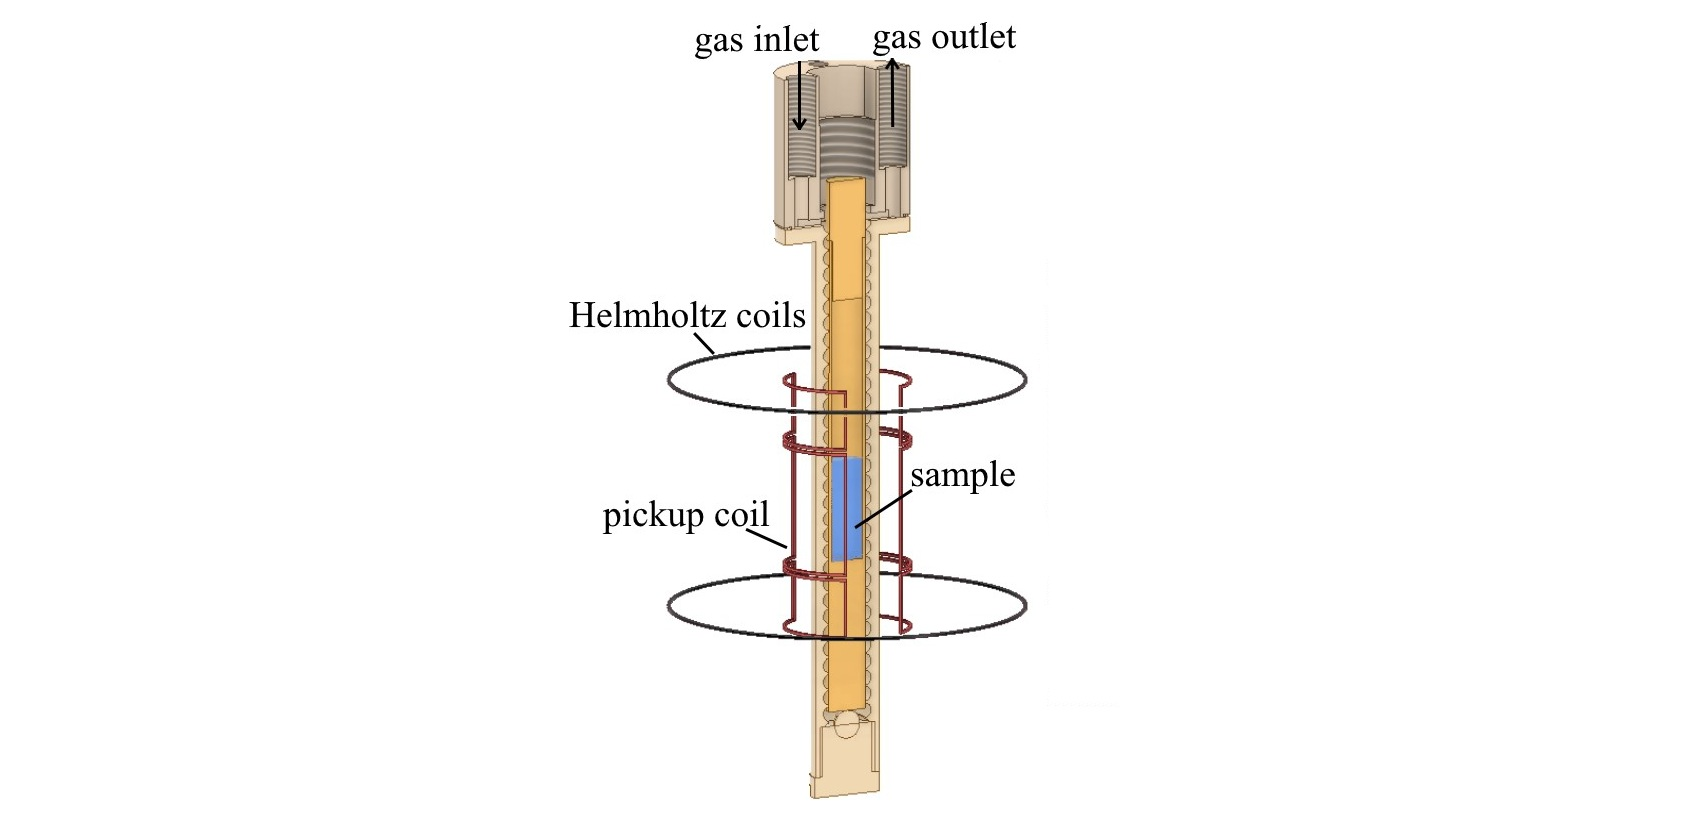
\includegraphics[width=\linewidth]{figures/VTII-schematic.png}
    \caption{The methanol sample (blue) sits at the center of the three-coil \ch{Nb} saddle-pair pickup (red).
    Helmholtz coils (black) fine-tune the bias magnetic field.
    Adapted from Ref.\,\cite{Walter2025_CASPErLFthermal} with permission.}
    \label{fig:VTII-Helmholtz_coil}
\end{figure}

At thermal equilibrium in the bias magnetic field $B_0$, the proton spins acquire a net longitudinal magnetization
\begin{equation}
    M_0 = \frac{n\,\gamma^2\hbar^2\,I(I+1)\,B_0}{3\,k_B\,T}
    \,,\label{eq:M0}
\end{equation}
where $n=\SI{6.0e22}{\cm^{-3}}$ is the proton number density of liquid methanol, $\gamma = 2\pi\times\SI{42.577}{\MHz/\tesla}$ is the proton gyromagnetic ratio, $I=1/2$ is the proton nuclear spin, $k_B$ is the Boltzmann constant, and $T$ is the sample temperature.
At $B_0 = \SI{31.67}{\milli\tesla}$ and $T \approx \SI{180}{\kelvin}$, the thermal polarization is $\approx\num{1.8e-7}$ and $M_0 \approx \SI{1.5e-04}{\ampere/\meter} = \SI{1.9e-10}{\tesla}/\mu_0$\,\cite{Zhang2026_Dissertation_ipynb_3_experiment}. 

\subsection{Pickup coil}\label{sec:apparatus:pickup}

A \ch{Nb} pickup coil mounted on the outside of the VTI in the L\ch{He} bath detects the transverse magnetization of the sample.
The coil consists of three saddle-pair coils in a gradiometer configuration: the area of the central coil is twice that of the two outer coils, and the coils are wound in opposing senses so that far-field flux contributions cancel.
The height of the central coil is \SI{24}{\milli\meter}, while the two outer coils are \SI{12}{\milli\meter} high.
The radii of all coils is \SI{14}{\milli\meter}.
The open angle of the each of the saddle-pair coils is \SI{120}{\degree}.
The filling factor---the fraction of the coil volume occupied by the sample---is approximately \SI{8}{\%}\,\cite{Zhang2026_Dissertation_ipynb_3_experiment}. 
The pickup coil geometry and pulsed-NMR scheme are illustrated in Figure~\ref{fig:VTII-Helmholtz_coil}.

\begin{figure}[htb]
    \centering
    \includegraphics[width=0.8\textwidth]{works/master-thesis/figures/02_Apparatus/Gradiometer_and_Sample_20220903.png}
    \caption{(a) Simplified schematic of gradiometer and sample positioned at the center.
    (b) Details of gradiometer loop connection showing the three-coil saddle-pair configuration with opposing windings for noise rejection.}
    \label{fig:gradiometer_sample}
\end{figure}



\subsection{SQUID detector}\label{sec:apparatus:squid}

Magnetic flux in the pickup coil is coupled into a direct-current superconducting quantum interference device (dc-SQUID), as shown in Figure~\ref{fig:squid_schematic}.
The SQUID circuit is enclosed in a \ch{Nb} capsule for shielding and protection from external disturbances.
The SQUID converts magnetic flux into electrical signals through the combination of flux quantization and Josephson tunneling effects, offering exceptional sensitivity for weak magnetic signals\,\cite{Mitchell2020_MagSensors}. 
SQUID is operated in flux-locked-loop (FLL) mode during measurements, i.e., a feedback voltage is applied to the SQUID to maintain the amount of magnetic flux in coils so that it remains at the linear operating point of its $V-\Phi$ characteristic, as illustrated in Figure~\ref{fig:squid_schematic}.
The feedback voltage is the measured output. 

\begin{figure}[htb]
    \centering
    \includegraphics[width=\textwidth]{works/master-thesis/figures/02_Apparatus/SQUID_Schematic_VPhi_FLL.png}
    \caption{(a) $V-\Phi$ characteristic of dc-SQUID showing the operating point W where the feedback voltage has approximately linear dependence on magnetic flux.
    (b) Direct-coupled FLL circuit with built-in pre-amplifier and integrator for maintaining the SQUID at the linear operating point.}
    \label{fig:squid_schematic}
\end{figure}

% The relationship between the magnetic flux coupled to the SQUID and the feedback voltage is given by Equation~\eqref{eq:squidpickup}, where the conversion factor depends on the coupling strengths and feedback parameters summarized in Table~\ref{tab:SQUID_params}.


The feedback voltage $V_\mathrm{f}$ is related to the magnetic flux in the pickup coil $\Phi_\mathrm{pick}$ by
\begin{equation}
    V_\mathrm{f}
    = \frac{R_\mathrm{f}}{M_\mathrm{f}}\,\frac{M_\mathrm{in}}{L_\mathrm{pick}+L_\mathrm{in}}\,\Phi_\mathrm{pick}
    = \varepsilon\,\Phi_\mathrm{pick}
    \,,\label{eq:squidpickup}
\end{equation}
where $R_\mathrm{f}$ is the feedback resistance, $M_\mathrm{f}$ is the feedback-coil mutual inductance, $M_\mathrm{in}$ is the mutual inductance between pickup and SQUID input coils, and $L_\mathrm{pick}$, $L_\mathrm{in}$ are the respective coil inductances.
The relavant parameters are summarized in Table~\ref{tab:SQUID_params}. 
% The conversion factor $\varepsilon \approx \SI{0.549}{\milli\volt/\Phi_0}$, where $\Phi_0$ is the magnetic flux quantum.

\begin{table}[ht]
    \centering
    \caption{Properties of the dc-SQUID sensor used in the measurements\,\cite{Zhang2026_Dissertation_ipynb_3_experiment}.}
    \begin{tabular}{lc}
        \hline\hline
        Pickup coil inductance ($L_\mathrm{pick}$) & \SI{553}{\nH} \\[0.5ex]
        SQUID input coil inductance ($L_\mathrm{in}$) & \SI{400}{\nH} \\[0.5ex]
        Mutual inductance ($M_\mathrm{in}$) & \SI{3.98}{\nH} \\[0.5ex]
        Feedback-coil inductance ($M_\mathrm{f}$) & \SI{22.83}{\Phi_0/\mA} \\[0.5ex]
        Feedback resistance ($R_\mathrm{f}$) & \SI{3}{\kohm} \\[0.5ex]
        Conversion factor ($\varepsilon$) & \SI{0.549}{\milli\volt/\Phi_0} \\[0.5ex]
        \hline\hline
    \end{tabular}
    \label{tab:SQUID_params}
\end{table}

The detection chain is also characterized by the transfer coefficient $\beta$, defined as the ratio of the SQUID feedback-voltage amplitude $V_\perp$ to the transverse sample magnetization $\mu_0 M_\perp$:
\begin{equation}
    \beta = \frac{V_\perp}{\mu_0\,M_\perp}
    \,.\label{eq:beta}
\end{equation}
The transfer coefficient was determined at each scan step from the feedback voltage following a $\pi/2$ pulse, for which $M_\perp = M_0$.
The average value is $\beta \approx \SI{4}{\milli\volt/\nano\tesla}$.

The SQUID output is fed into a Zurich Instruments MFLI Lock-in Amplifier (LIA), which demodulates the signal into in-phase ($I$) and quadrature ($Q$) channels.
The outputs of the two channels are recorded at a sampling frequency of \SI{13.4}{\kHz} and is used to generate spectra via fast Fourier transformation (FFT).

During ALP-search measurements the SQUID and FLL electronics are battery-powered to avoid electromagnetic interference from the mains.
All other electronics (lock-in amplifier, field-ramp supply) are outside the Faraday cage; only shielded Bayonet Neill-Concelman (BNC) cables penetrating the cage are used to carry signals.

\subsection{Experimental control and data acquisition}\label{sec:apparatus:control}

Comprehensive centralized control of the CASPEr-Gradient-LF apparatus is implemented in Python to coordinate the complex timing requirements of pulsed-NMR experiments and manage communication between diverse hardware components.
This control system enables synchronized operation of shim coils, rf pulse generation, and SQUID data acquisition.

The main functions of the control system include:

\begin{enumerate}
    \item \textbf{Magnet and shim control:}
    \begin{enumerate}
        \item Remote switching of shim power supply on and off
        \item Connection and disconnection of communication between power supply and shim coils
        \item Real-time setting of shim currents to desired values, with optional heater control for current stabilization
    \end{enumerate}
    \item \textbf{Pulse generation and timing:}
    \begin{enumerate}
        \item Command interface for injecting radiofrequency pulses
        \item Recording rf pulse timing via oscilloscope into HDF5 format
        \item Analysis of function generator data and pulse characterization
    \end{enumerate}
    \item \textbf{Data acquisition and processing:}
    \begin{enumerate}
        \item Recording SQUID data and automated creation of HDF5 files for storage
        \item Real-time analysis and monitoring of acquired signals
        \item Generation and analysis of power spectral densities
    \end{enumerate}
\end{enumerate}

The control system orchestrates multiple measurement schemes including pulsed-NMR diagnostics for sample characterization, automated shimming procedures with feedback optimization, axion wind measurements, and magnetic field monitoring.
Additionally, the system includes capabilities for NMR kinetic simulations, stochastic axion wind simulations, apparatus properties computation, and synchronized file management across multiple terminals.




\section{Sensitivity}\label{sec:experiment:sensitivity}

The transverse magnetization induced by the ALP field couples to the pickup coil and SQUID. 
Due to the stochastic nature of the ALP field, the signal can vary significantly over time and is therefore characterized by its average power rather than a deterministic amplitude.
In addition to the ALP coherence time $\tau_a$, the signal is also affected by the sample relaxation times $T_2^*$. 
When $T_2^* \ll \tau_a$, the amplitude of the signal, characterized by the tipping angle $\xi$, is limited by the sample relaxation time, and it grows as
\begin{equation}
    \xi(t) = (1 - e^{-t/T_2^*}) \Omega_a T_2^*
    \,,\label{eq:s_t_T2star_ll_tau_a}
\end{equation}
and saturates at $t\gg T_2^*$. 
When $T_2^* \gg \tau_a$, the signal first grows linearly at $t\ll\tau_a$, and then grows as $\sim (t\tau_a)^{1/2}$ at $\tau_a<t<T_2^*$ like a random walk\,\cite{Gramolin2022Feb_SpectralSignatures, Yuzhe2023_FrequencyScanning}, saturating at $t\gg T_2^*$.
An analytical expression for the signal in this regime derived from numerical simulations is
\begin{equation}
    \xi(t) = \left(1 - \exp{\left(\frac{-t}{\frac{1}{2}T_2^*}\right)}\right)^{1/2} \Omega_a \left(T_2^*\tau_a\right)^{1/2}
    \,.\label{eq:xi_t_T2star_gg_tau_a}
\end{equation}
% When the measurement duration $T$ and sample relaxation time $T_2^*$ are much longer than the ALP coherence time $\tau_a$, the signal amplitude varies randomly over time.
% Hence, 
% When $T_2^*\gg\tau_a$, the final signal amplitude $\approx \Omega_a (T_2^*\tau_a)^{1/2}$. And we also found that the signal grows up with $\sim (t\tau_a)^{1/2}$ at first. So we can use
% $s(t) = \left(1 - \exp{\left(\frac{-t}{\frac{1}{2}T_2^*}\right)}\right)^{1/2} \Omega_a (T_2^*\tau_a)^{1/2}$
% to describe the signal. 
% Beside, for the sack of simplicity in numerical calculations, we can use this formula to approximate the signal under any circumstances
To unify the two regimes, we introduce a parameter $x$ that interpolates between the two limits:
\begin{equation}
    \xi(t) = \left(1 - \exp{\left(\frac{-t}{x T_2^*}\right)}\right)^{x} \Omega_a T_2^* \left(\frac{\tau_a}{\tau_a + T_2^*}\right)^{1/2}
    \,.\label{eq:xi_t_general}
\end{equation}
For most measurements, $T_2^*,\, \tau_a \ll T$ holds, so the ALP-induced signal amplitude is approximately 
\begin{equation}
    \xi = \Omega_a T_2^* \left(\frac{\tau_a}{\tau_a + T_2^*}\right)^{1/2}
    \,.\label{eq:xi_final}
\end{equation}
This tipping angle corresponds to a transverse magnetization $M_\perp = M_0 \sin{\xi} \approx M_0 \xi$ for small $\xi$, which is the case for the ALP-induced signal considering the expected Rabi frequencies in Equations~\eqref{eq:Omega_a_MW} and~\eqref{eq:Omega_a_EH}. 
% The signal measured is therefore proportional to the ALP-induced
% Consequently, the ALP-induced signal is proportional to the ALP-induced tipping angle $\xi$ and the transverse magnetization $M_\perp$.
Taking Equations~\eqref{eq:beta} and \eqref{eq:xi_final} into account, the following relationship is obtained:
\begin{equation}
    V_a = \beta\,\mu_0 M_0 \Omega_a T_2^* \left(\frac{\tau_a}{\tau_a + T_2^*}\right)^{1/2} \propto g_{\mathrm{aNN}} \left(\frac{\tau_a}{\tau_a + T_2^*}\right)^{1/2}
    \,,\label{eq:Va_gaNN_Tcoh}
\end{equation}
where $V_a$ is the SQUID feedback voltage corresponding to the ALP-induced transverse magnetization. 
In the following discussion, the experimental parameters $\beta$ and $M_0$ are treated as constants and therefore omitted for simplicity, and the ALP-induced signal is expressed as $g_{\mathrm{aNN}} T_{\mathrm{coh}}$ where $T_{\mathrm{coh}} = \left(\tau_a T_2^*/\left(\tau_a + T_2^*\right)\right)^{1/2}$ is the effective coherence time of the ALP-induced signal. 

% This tipping angle can be connected to a the observable by a constant coefficient since 
% Using Equations~??, the average ALP-induced flux power is
% \begin{align}
%     \langle \Phi_a^2 \rangle
%     =\frac{1}{2}(\beta\, u_n\, \mu_0 M_0 \Omega_a)^2 \left\{
%     \begin{array}{cl}
%     \tau_a T_2^* ,
%     &  \tau_a \ll T_2^*\\[6pt]
%     \frac{\tau_a^2}{\pi} ,
%     &  T_2^*\ll\tau_a \ll T_2\\[6pt]
%     T_2^2 ,
%     &  T_2 \ll \tau_a
%     \end{array} \right.
%     \,. \label{eq:Phia2}
% \end{align}
The signal amplitude in the power spectral density (PSD) is
\begin{align}
    \mathrm{PSD} = \frac{\left(g_{\mathrm{aNN}} T_{\mathrm{coh}}\right)^2}{\Delta\nu}
    \,,
    \label{eq:S_PSD}
\end{align}
where $\Delta\nu$ is the expected signal linewidth, which is determined by the narrower of the ALP linewidth $\Delta\nu_a = 1/(\pi \tau_a)$ and the NMR linewidth $\Delta\nu_n = 1/(\pi T_2^*)$.
Hence, $\Delta\nu$ can be expressed as 
\begin{equation}
    \Delta\nu = \frac{1}{\pi} \frac{1}{\tau_a + T_2^*}
    \,.\label{eq:Gamma_signal}
\end{equation}
% Assuming 
% Depending on which linewidth is narrower,
% \begin{equation}
%     \Delta\nu = \left\{
%     \begin{array}{cl}
%     \Delta\nu_a ,
%     &  \Delta\nu_a \ll \Delta\nu_{n}\\[4pt]
%     \Delta\nu_a ,
%     &  \Delta\nu_a \ll \Delta\nu_{n}\\[4pt]
%     \Delta\nu_{n},
%     & \Delta\nu_a  \gg \Delta\nu_{n}
%     \end{array} \right.
%     \,.\label{eq:Gamma_signal}
% \end{equation}
Within a spectral bin of width $\Delta\nu$, the number of PSD values available for averaging from a measurement of duration $T$ is
\begin{equation}
    N_{\Delta\nu} = T \Delta\nu \gg 1
    \,,\label{eq:NGamma}
\end{equation}
assuming that the measurement duration is much longer than the ALP coherence time and the sample relaxation time. 
The noise, characterized by standard deviation, is
\begin{equation}
    \sigma = \sqrt{\frac{1}{T \Delta\nu}}\,\sigma_{0}
    \,,\label{eq:sigma}
\end{equation}
where $\sigma$ and $\sigma_{0}$ are the noise with and without averaging, respectively. 
Since $N_{\Delta\nu} \gg 1$, the noise distribution approaches a Gaussian distribution according to the central limit theorem. 
% The $g_{\mathrm{aNN}}$ sensitivity can be derived by the signal-to-noise ratio (SNR) in the PSD. 
The coupling strength $g_{\mathrm{aNN}}$ that a \SI{5}{\sigma} signal correspond to can be found by the SNR condition
\begin{equation}
    \frac{\mathrm{PSD}}{\sigma} = 5
    \,.\label{eq:SNR_condition}
\end{equation}
which can be expanded by Equations~\eqref{eq:S_PSD}, \eqref{eq:Gamma_signal}, and \eqref{eq:sigma} to
\begin{equation}
    \frac{g_{\mathrm{aNN}}^2 T_{\mathrm{coh}}^2 T^{1/2} }{\Delta\nu^{1/2}\sigma_0} = 5
    \,.\label{eq:SNR_condition_expanded}
\end{equation}
Hence, the $g_{\mathrm{aNN}}$ sensitivity is
\begin{equation}
    \left|g_{\mathrm{aNN}}\right| \propto 
    T^{-1/4} 
    \left(T_2^*\right)^{-1}   
    \tau_a^{-1/2} 
    \left(T_2^* + \tau_a\right)^{1/4} 
    \,.\label{eq:g_aNN_sensitivity}
\end{equation}
Here a constant factor of $5^{1/2}\,\sigma_0^{1/2} \pi^{-1/4}$ is dropped since only the scaling of $g_{\mathrm{aNN}}$ with $\tau_a$, $T_2^*$, and $T$ is of interest. 
In terms of the two extreme regimes of $\tau_a$ relative to $T_2^*$ and $T_2$, the sensitivity can be expressed as
\begin{equation}
    \left|g_{\mathrm{aNN}}\right| \propto
    \left\{
    \begin{array}{cl}
    T^{-1/4}\, \left(T_2^*\right)^{-1}\, \tau_a^{-1/4}  ,
    &  T_2^* \ll \tau_a \\[6pt]
    T^{-1/4}\, \left(T_2^*\right)^{-3/4}\, \tau_a^{-1/2}   ,
    &  T_2^* \gg \tau_a
    \end{array} \right.
    \,. \label{eq:g_aNN_sensitivity_2regimes}
\end{equation}
The implications from Equation~\eqref{eq:g_aNN_sensitivity_2regimes} can be summarized as follows:
\begin{enumerate}
    \item When measurement duration $T$ is much longer than the sample relaxation time $T_2^*$ and the ALP coherence time $\tau_a$, the sensitivity is dominated by the term $T^{-1/4}$, indicating a slower improvement with increasing measurement duration. 
    \item The sensitivity improves with longer sample relaxation time $T_2^*$. The improvement is more significant when $T_2^* \ll \tau_a$. 
\end{enumerate}





\section{Scanning}\label{sec:experiment:scanning}

\subsection{Procedure}\label{sec:experiment:scanning:procedure}

The CASPEr-Gradient-Lowfield experiment scans the ALP-mass parameter space by sweeping the magnitude of $\mathbf{B}_0$, which tunes the Larmor frequency of the sample to a series of values $\nu_i \in [\nu_{\mathrm{start}},\,\nu_{\mathrm{end}}]$.
One step of the scan consists of:
\begin{enumerate}[label=\Alph*.]
    \item Pulsed-NMR measurement to determine the resonance frequency and the effective linewidth ($T_2^*$).
    \item Spin-echo measurement to determine $T_2$.
    \item Data acquisition with the SQUID magnetometer---no transverse pulse applied---to record the ALP-signal channel over the measurement duration $T$.
    % \item Fourier transform of the magnetometer data to produce a power spectrum.
    % \item Binning of PSD values within frequency bins of width $\Delta\nu$, and averaging to reduce noise.
    % \item Statistical analysis of binned PSD values (e.g., histogram comparison with the expected noise distribution) to identify DM-candidate frequencies.
    % \item If a candidate is found: repeat the measurement at the same field value and perform additional checks.
    % \item If no candidate is found: record the exclusion contour for this frequency step and ramp $\mathbf{B}_0$ to the next value.
    \item Ramp $\mathbf{B}_0$ to the next value. 
\end{enumerate}
% The procedure is illustrated in Figure~\ref{fig:CASPEr_Procedure}.
% A significant excess surviving repeated measurement can be tested further.
% \begin{figure}[htb]
%     \centering
%     \includegraphics[width=0.8\linewidth]{works/frequency-scanning/CASPEr_Procedure_20230311.png}
%     \caption{Schematic of the experimental procedure.
%     (a) One step of the scan: pulsed-NMR diagnostics, free-precession data acquisition, PSD computation and binning, and statistical analysis using a histogram of PSD values.
%     (b) Example decay spectra (blue curves) and the resulting sensitivity region in the ALP mass-coupling space (reddish area) after scanning over a frequency range.
%     Reproduced from Ref.\,\cite{Yuzhe2023_FrequencyScanning}, originally prepared by the author.}
%     \label{fig:CASPEr_Procedure}
% \end{figure}
The frequency-scan-step size is set by the sensitive bandwidth of a single step.
% An experiment is sensitive to signals within a bandwidth equal to the maximum of $\Delta\nu_n$ and $\Delta\nu_a$ around a given Larmor frequency. 
The sensitive bandwidth is a bandwidth around the Larmor frequency where the experiment is approximately equally sensitive to ALP signals. 
It can be considered by the NMR linewidth, the ALP linewidth, and the noise profile. 
On one hand, in terms of non-amplifiable noise (white noise, flat in spectrum), the experiment is sensitive in bandwidth approximately equal to the maximum of the NMR linewidth and the ALP linewidth.
On the other hand, in terms of noise amplified by NMR, the experiment is equally sensitive in bandwidth much larger than the NMR linewidth. 
Choosing a step size larger than sensitive bandwidth leaves gaps in sensitivity; choosing a smaller step size multiplies the number of steps and the dead time between steps without improving sensitivity.
Therefore, the scan-step size is set to be approximately equal to the sensitive bandwidth of a single step.
Examples of amplifiable and non-amplifiable noises are illustrated in Figure~\ref{fig:scan-flat_peak_sensi}.
For CASPEr-Gradient experiments, the dominant noise type is non-amplifiable noise, which is assumed for the following discussion.

\begin{figure}[htb]
    \centering
    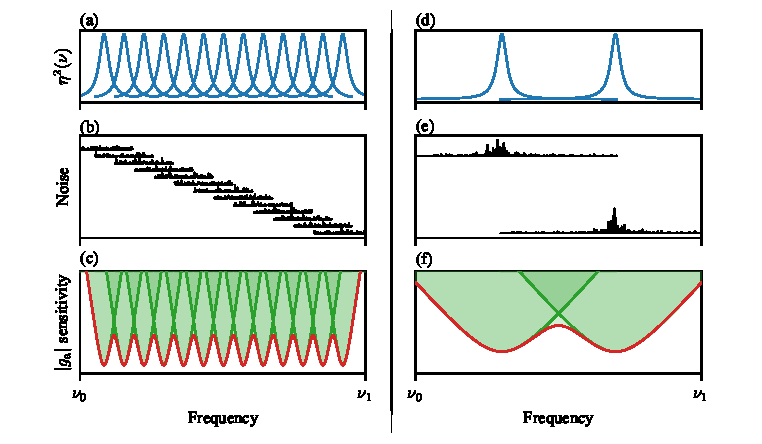
\includegraphics[width=\linewidth]{figures/scan-flat_peak_sensi.pdf}
    \caption{Examples of experiments scanning over the frequency range $[\nu_0,\,\nu_1]$.  Each of the spectra corresponds to one scan step over a certain frequency range. 
    Left column: Dominance of non-amplifiable noise.
    Right column: Dominance of amplifiable noise.
    Rows (top to bottom): Frequency spectra of the square of magnetic signal amplification $\eta(\nu)$ in panels (a) and (d), PSD noise in panels (b) and (e), and the corresponding $g_\mathrm{a}$ sensitivity in panels (c) and (f). Offsets have been added to the noise spectra for clarity.
    The scan-step size is larger when amplifiable noise dominates due to the broader sensitivity bandwidth. 
    Adapted from Ref.\,\cite{YGK2026_CavityLumpedSpin}, originally prepared by the author.}
    \label{fig:scan-flat_peak_sensi}
\end{figure}



\subsection{Optimization of scanning}\label{sec:experiment:scanning:optimization}

Two questions arise after the previous discussion:
What is the figure of merit for a scanning strategy? 
How to optimize the scanning strategy to maximize the figure of merit? 
The choice of figure of merit is arbitrary, but a natural choice is the area covered in the $\log|g_{\mathrm{aNN}}|$--$\log\nu$ mass-coupling parameter space.
Given a fixed total measurement time, the relaxation times $T_2^*$ can be tuned to maximize the parameter space coverage.
% A long relaxation time $T_2^*$ improves sensitivity at each frequency step, but it also decreases the scan-step size, which increases the number of steps and decreases the measurement time per step. 
A short relaxation time $T_2^*$ may allow for a larger scan-step size and less total steps, and therefore increases the measurement time per step. 
However, as can be estimated from the scalings in Equation~\eqref{eq:g_aNN_sensitivity_2regimes}, the increase in the measurement time per step is not sufficient to compensate for the decrease in relaxation time in terms of sensitivity.

A more careful analysis of the trade-off between relaxation time and measurement time per step is given as follows.
With fixed total measurement time $T_{\mathrm{tot}}$, the dwell time can be chosen to be proportional to the ALP coherence time: $T \propto \tau_a \propto \nu^{-1}$.\footnote{Measurement time can also be allocated uniformly across frequency steps, which makes no significant difference in the final sensitivity. A quantitative comparison of the two ways of allocation is given in Ref.\,\cite{Yuzhe2023_FrequencyScanning}.}
The scan rate can be found as
\begin{equation}
    \frac{d\nu}{dt} = \frac{\Delta\nu}{T} =\frac{\Delta\nu}{\kappa \tau_a} 
    % = \left(\kappa \tau_a \left(T_2^* + \tau_a\right)\right)^{-1}
    \,,\label{eq:scan_rate}
\end{equation}
where $\kappa$ is a constant going to be determined later by the total measurement time and the scan range. 
The two regimes in Equation~\eqref{eq:g_aNN_sensitivity_2regimes} are discussed separately. 
% \textbf{Regime (1): $ T_2^* \ll \tau_a $}
In the $ T_2^* \ll \tau_a $ regime, $\Delta\nu = 1 / (\pi \tau_a)$. 
A shorter $T_2^*$ does not allow for a larger scan-step size, so the sensitivity is worse when $T_2^*$ is shorter. 
% Using $\tau_a = Q_a / \nu$ and Equation~\eqref{eq:scan_rate}, the scan rate becomes
% \begin{equation}
%     \frac{d\nu}{d t} = \frac{\nu^2}{\pi \kappa Q_a^2 }
%     \,.\label{eq:scan_rate_regime1}
% \end{equation}
% which leads to
% \begin{equation}
%     \int_{\nu_\mathrm{start}}^{\nu_\mathrm{end}} \nu^{-2} d\nu = \int_{0}^{T_\mathrm{tot}} \frac{1}{\pi \kappa Q_a^2 } d t
%     \,.\label{eq:scan_rate_regime1_integral}
% \end{equation}
% $\kappa$ can be solved as
% \begin{equation}
%     \kappa = \frac{T_\mathrm{tot}}{\pi Q_a^2 } \frac{\nu_\mathrm{start} \nu_\mathrm{end}}{\nu_\mathrm{end}-\nu_\mathrm{start}}
%     \,.\label{eq:kappa_regime1}
% \end{equation}
% Usually, the scanning covers orders of magnitudes, so $\nu_\mathrm{end} \gg \nu_\mathrm{start}$ is typical.
% In this case, the sensitivity in this regime is ...
In the other regime where $ T_2^* \gg \tau_a $, $\Delta\nu = 1 / (\pi T_2^*)$. 
Using $\tau_a = Q_a / \nu$ and Equation~\eqref{eq:scan_rate}, the scan rate becomes
\begin{equation}
    \frac{d\nu}{d t} = \frac{\nu}{\pi \kappa Q_a T_2^* }
    \,.\label{eq:scan_rate_regime1}
\end{equation}
which leads to
\begin{equation}
    \int_{\nu_\mathrm{start}}^{\nu_\mathrm{end}} \nu^{-1} d\nu = \int_{0}^{T_\mathrm{tot}} \frac{1}{\pi \kappa Q_a T_2^* } d t
    \,.\label{eq:scan_rate_regime1_integral}
\end{equation}
$\kappa$ can be solved as
\begin{equation}
    \kappa = \frac{T_\mathrm{tot}}{\pi Q_a T_2^* } \ln\left(\frac{\nu_\mathrm{end}}{\nu_\mathrm{start}}\right) \propto T_\mathrm{tot} \left(T_2^*\right)^{-1}
    \,.\label{eq:kappa_regime2}
\end{equation}
Consider Equations~\eqref{eq:g_aNN_sensitivity_2regimes} and \eqref{eq:kappa_regime2} and omitting the constant factors, the sensitivity in this regime is 
\begin{equation}
    \left|g_{\mathrm{aNN}}\right| \propto
    T_{\mathrm{tot}}^{-1/4}\, \left(T_2^*\right)^{-1/2}\, \tau_a^{-1/2}
    \,. \label{eq:g_aNN_sensitivity_scan_regime2}
\end{equation}
From Equation~\eqref{eq:g_aNN_sensitivity_scan_regime2}, the sensitivity still improves with longer $T_2^*$, which is consistent with the estimation in previous discussion.

% Maximizing the sensitive area in the $\log\nu$--$\log|g_{\mathrm{aNN}}|$ parameter space over the full scan determines the optimal exponent $n$.
% The derivation is given in Appendix~\ref{app:dwell_time}; the result is $n=0$ (uniform dwell time) for regimes~(1)--(3) and $n=-1$ (dwell time decreasing as $1/\nu$) for regime~(4).

% With optimal dwell-time allocation, the scanning sensitivity is
% \begin{equation}
%     |g_{\mathrm{aNN}}| \geqslant
%     \begin{cases}
%     \eta
%     \left(\frac{T_{\mathrm{tot}}}{Q_a\ln\left(\nu_{\mathrm{end}}/\nu_{\mathrm{start}} \right)}\right)^{-1/4}
%     (T_2^*)^{-3/4}\, \tau_a^{-1/2},
%     & \substack{\tau_a\ll T_2^* \text{ or}\\ T_2^*\ll\tau_a\ll T_2} \\[10pt]
%     \eta
%     \left(\frac{\pi^2 T_{\mathrm{tot}}}{Q_a\ln\left(\nu_{\mathrm{end}}/\nu_{\mathrm{start}} \right)}\right)^{-1/4}
%     (T_2^*)^{-3/4}\, T_2^{-1}\, \tau_a^{1/2},
%     & \substack{T_2^* \ll T_2 \ll \tau_a \text{ or}\\ T_2^*=T_2 \ll \tau_a}
%     \end{cases}
%     \,.\label{eq:gaNN_Ttot_optimal}
% \end{equation}

% Several conclusions follow directly:
% \begin{itemize}
%     \item \textbf{Time scaling.}
%     The sensitivity scales as $T_{\mathrm{tot}}^{-1/4}$ in all regimes, a consequence of the long-dwell-time limit $T \gg \tau_a,\,T_2^*,\,T_2$\,\cite{CASPErProposal2014,Aybas_2021_Quantum_sensitivity}.
%     An order-of-magnitude increase in measurement time improves the exclusion bound by only a factor $10^{1/4}\approx1.8$.

%     \item \textbf{Effect of $T_2^*$.}
%     Longer $T_2^*$ is beneficial in all regimes.
%     When $\tau_a \ll T_2^*$, it increases the rms\ tipping angle and narrows the signal linewidth.
%     When $T_2^* \ll \tau_a$, it increases the fraction $u_n$ of spins on resonance.

%     \item \textbf{Effect of $T_2$.}
%     Longer $T_2$ improves sensitivity in the regime $T_2 \ll \tau_a$, where $T_2$ directly limits the rms\ tipping angle.
% \end{itemize}

% The sensitivity plots computed with uniform ($n=0$) and frequency-adaptive ($n=-1$) dwell-time allocation for an example scan range $\nu_{\mathrm{end}}/\nu_{\mathrm{start}}=10$ are shown in Figure~\ref{fig:UniVsAdpt}.
% The area covered in the $\log\nu$--$\log|g_{\mathrm{aNN}}|$ plane is larger with optimal $n$.

% \begin{figure}[htb]
%     \centering
%     \includegraphics[width=.7\linewidth]{works/frequency-scanning/UniVsAdpt_20230412-3.png}
%     \caption{Sensitivity plots on a log-log scale for two dwell-time allocation schemes: uniform ($n=0$) and frequency-adaptive ($n=-1$).
%     The shaded regions indicate the parameter space accessible to the experiment.
%     The coupling strength is normalized in each regime so that the highest point equals 1.
%     The scan range is $\nu_{\mathrm{end}}/\nu_{\mathrm{start}}=10$.
%     Reproduced from Ref.\,\cite{Yuzhe2023_FrequencyScanning}, originally prepared by the author.}
%     \label{fig:UniVsAdpt}
% \end{figure}

In summary, the optimal strategy for a frequency-scanning ALP search is to work at the maximum achievable $T_2^*$.

